% =============================================================================
% Cross-Paper Pipeline Figure for NSF Project
% P0 (Definition) -> P1 (Identification) -> P3 (Adversarial Evaluation)
%
% Usage: % =============================================================================
% Cross-Paper Pipeline Figure for NSF Project
% P0 (Definition) -> P1 (Identification) -> P3 (Adversarial Evaluation)
%
% Usage: % =============================================================================
% Cross-Paper Pipeline Figure for NSF Project
% P0 (Definition) -> P1 (Identification) -> P3 (Adversarial Evaluation)
%
% Usage: % =============================================================================
% Cross-Paper Pipeline Figure for NSF Project
% P0 (Definition) -> P1 (Identification) -> P3 (Adversarial Evaluation)
%
% Usage: \input{shared/figures/fig_pipeline.tex}
% Requires: \usepackage{tikz} in the parent document
% =============================================================================
\begin{figure*}[t]
\centering
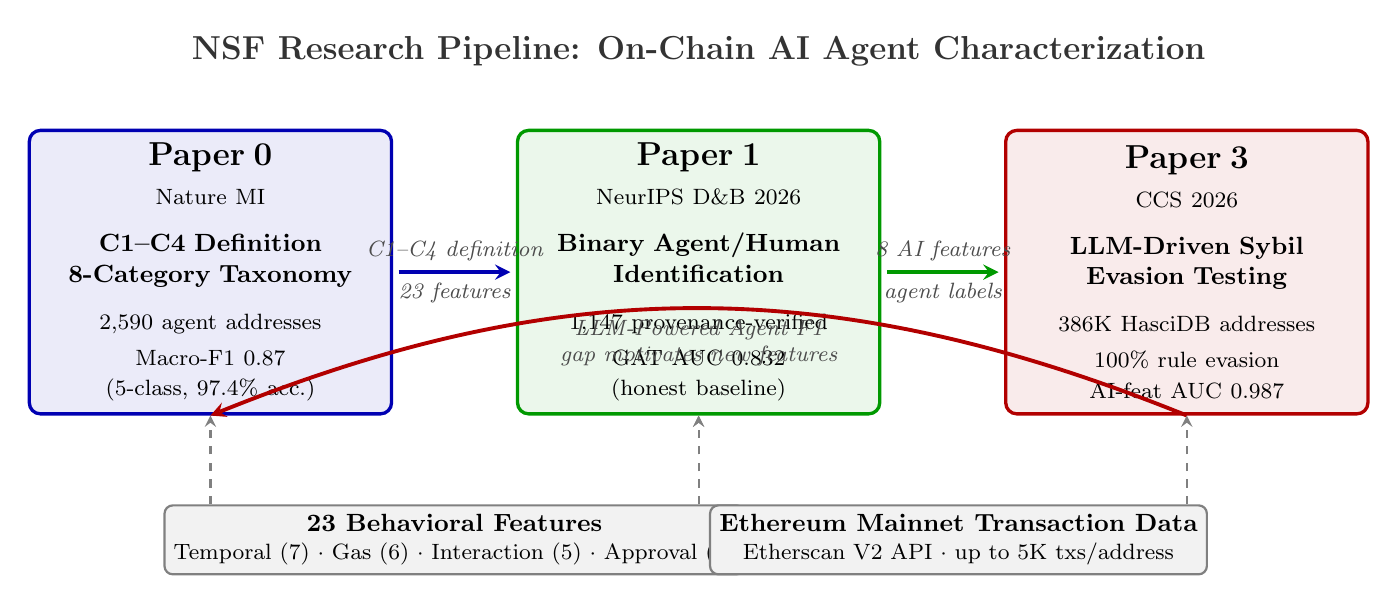
\begin{tikzpicture}[
    % Node styles
    paperbox/.style={
        rectangle,
        rounded corners=4pt,
        draw=#1,
        line width=1.2pt,
        fill=#1!8,
        minimum width=4.6cm,
        minimum height=3.6cm,
        text width=4.2cm,
        align=center,
        font=\small
    },
    databox/.style={
        rectangle,
        rounded corners=3pt,
        draw=black!50,
        line width=0.8pt,
        fill=black!5,
        minimum width=5cm,
        minimum height=0.8cm,
        align=center,
        font=\small
    },
    arrow/.style={
        ->,
        >=stealth,
        line width=1.4pt,
        color=#1
    },
    dataarrow/.style={
        ->,
        >=stealth,
        line width=0.8pt,
        dashed,
        color=black!50
    },
    label/.style={
        font=\footnotesize\itshape,
        text=black!70
    }
]

% ===== Paper boxes =====

% Paper 0
\node[paperbox=blue!70!black] (p0) at (0, 0) {
    \textbf{\large Paper 0}\\[3pt]
    {\footnotesize Nature MI}\\[6pt]
    \textbf{C1--C4 Definition}\\
    \textbf{8-Category Taxonomy}\\[6pt]
    {\footnotesize 2,590 agent addresses}\\[2pt]
    {\footnotesize Macro-F1 0.87}\\
    {\footnotesize (5-class, 97.4\% acc.)}
};

% Paper 1
\node[paperbox=green!60!black] (p1) at (6.2, 0) {
    \textbf{\large Paper 1}\\[3pt]
    {\footnotesize NeurIPS D\&B 2026}\\[6pt]
    \textbf{Binary Agent/Human}\\
    \textbf{Identification}\\[6pt]
    {\footnotesize 1,147 provenance-verified}\\[2pt]
    {\footnotesize GAT AUC 0.832}\\
    {\footnotesize (honest baseline)}
};

% Paper 3
\node[paperbox=red!70!black] (p3) at (12.4, 0) {
    \textbf{\large Paper 3}\\[3pt]
    {\footnotesize CCS 2026}\\[6pt]
    \textbf{LLM-Driven Sybil}\\
    \textbf{Evasion Testing}\\[6pt]
    {\footnotesize 386K HasciDB addresses}\\[2pt]
    {\footnotesize 100\% rule evasion}\\
    {\footnotesize AI-feat AUC 0.987}
};

% ===== Arrows between papers =====

\draw[arrow=blue!70!black] ([xshift=2pt]p0.east) -- ([xshift=-2pt]p1.west)
    node[midway, above, label] {C1--C4 definition}
    node[midway, below, label] {23 features};

\draw[arrow=green!60!black] ([xshift=2pt]p1.east) -- ([xshift=-2pt]p3.west)
    node[midway, above, label] {8 AI features}
    node[midway, below, label] {agent labels};

% ===== Feedback arrow P3 -> P0 =====

\draw[arrow=red!70!black, bend right=22] (p3.south) to
    node[midway, below, label, text width=6cm, align=center]
    {LLM-Powered Agent F1 gap motivates new features}
    (p0.south);

% ===== Shared data layer =====

\node[databox] (feat) at (3.1, -3.4) {
    \textbf{23 Behavioral Features}\\[-1pt]
    {\footnotesize Temporal (7) $\cdot$ Gas (6) $\cdot$ Interaction (5) $\cdot$ Approval (5)}
};

\node[databox] (data) at (9.5, -3.4) {
    \textbf{Ethereum Mainnet Transaction Data}\\[-1pt]
    {\footnotesize Etherscan V2 API $\cdot$ up to 5K txs/address}
};

% ===== Dashed arrows from data layer to papers =====

\draw[dataarrow] (feat.north -| p0) -- (p0.south);
\draw[dataarrow] (feat.north -| p1) -- (p1.south);
\draw[dataarrow] (data.north -| p1) -- (p1.south);
\draw[dataarrow] (data.north -| p3) -- (p3.south);

% ===== Title =====

\node[font=\large\bfseries, text=black!80] at (6.2, 2.8) {
    NSF Research Pipeline: On-Chain AI Agent Characterization
};

\end{tikzpicture}
\caption{Cross-paper pipeline. Paper~0 defines on-chain AI agents via four conditions (C1--C4) and validates an eight-category taxonomy on 2,590 addresses. Paper~1 uses the same 23 features for binary agent/human identification on 1,147 provenance-verified addresses (honest GAT AUC 0.832). Paper~3 tests whether LLM-driven Sybils can evade airdrop detectors; 8 AI-specific features from Paper~1 recover AUC 0.987 even after all HasciDB rules are defeated. The feedback arrow represents Paper~3's finding that the LLM-Powered Agent category (F1 = 0.528 in Paper~0) needs the 8 AI features to become distinguishable. Dashed arrows show shared data dependencies.}
\label{fig:pipeline}
\end{figure*}

% Requires: \usepackage{tikz} in the parent document
% =============================================================================
\begin{figure*}[t]
\centering
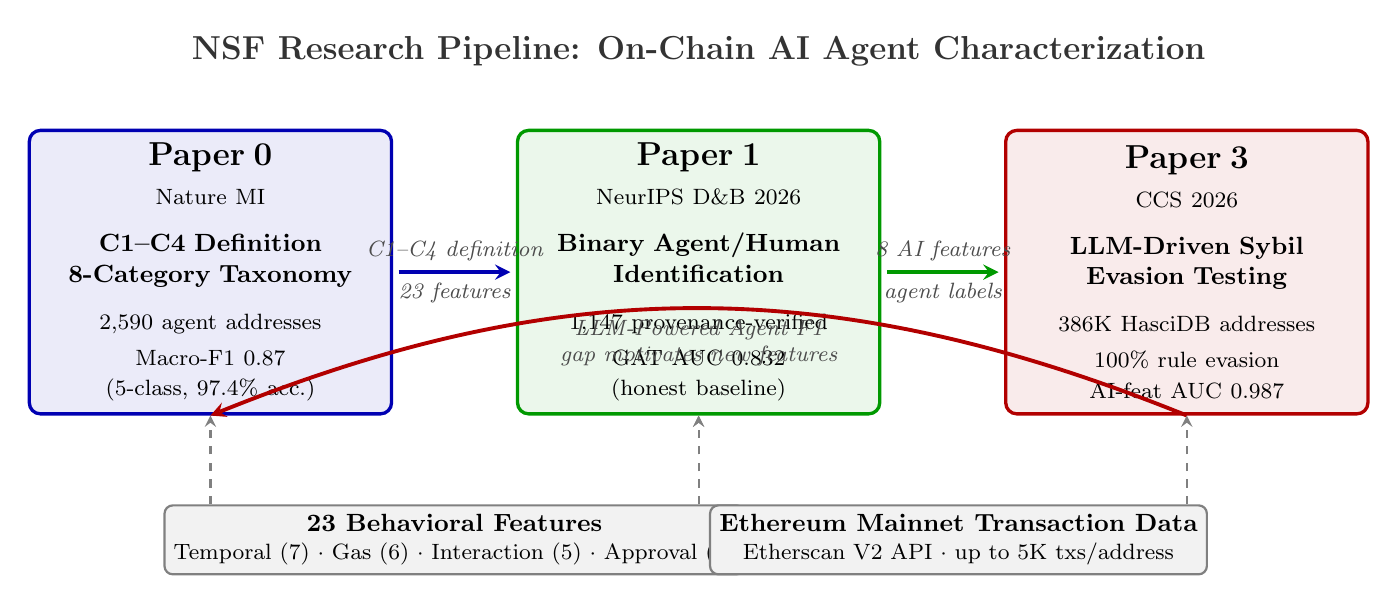
\begin{tikzpicture}[
    % Node styles
    paperbox/.style={
        rectangle,
        rounded corners=4pt,
        draw=#1,
        line width=1.2pt,
        fill=#1!8,
        minimum width=4.6cm,
        minimum height=3.6cm,
        text width=4.2cm,
        align=center,
        font=\small
    },
    databox/.style={
        rectangle,
        rounded corners=3pt,
        draw=black!50,
        line width=0.8pt,
        fill=black!5,
        minimum width=5cm,
        minimum height=0.8cm,
        align=center,
        font=\small
    },
    arrow/.style={
        ->,
        >=stealth,
        line width=1.4pt,
        color=#1
    },
    dataarrow/.style={
        ->,
        >=stealth,
        line width=0.8pt,
        dashed,
        color=black!50
    },
    label/.style={
        font=\footnotesize\itshape,
        text=black!70
    }
]

% ===== Paper boxes =====

% Paper 0
\node[paperbox=blue!70!black] (p0) at (0, 0) {
    \textbf{\large Paper 0}\\[3pt]
    {\footnotesize Nature MI}\\[6pt]
    \textbf{C1--C4 Definition}\\
    \textbf{8-Category Taxonomy}\\[6pt]
    {\footnotesize 2,590 agent addresses}\\[2pt]
    {\footnotesize Macro-F1 0.87}\\
    {\footnotesize (5-class, 97.4\% acc.)}
};

% Paper 1
\node[paperbox=green!60!black] (p1) at (6.2, 0) {
    \textbf{\large Paper 1}\\[3pt]
    {\footnotesize NeurIPS D\&B 2026}\\[6pt]
    \textbf{Binary Agent/Human}\\
    \textbf{Identification}\\[6pt]
    {\footnotesize 1,147 provenance-verified}\\[2pt]
    {\footnotesize GAT AUC 0.832}\\
    {\footnotesize (honest baseline)}
};

% Paper 3
\node[paperbox=red!70!black] (p3) at (12.4, 0) {
    \textbf{\large Paper 3}\\[3pt]
    {\footnotesize CCS 2026}\\[6pt]
    \textbf{LLM-Driven Sybil}\\
    \textbf{Evasion Testing}\\[6pt]
    {\footnotesize 386K HasciDB addresses}\\[2pt]
    {\footnotesize 100\% rule evasion}\\
    {\footnotesize AI-feat AUC 0.987}
};

% ===== Arrows between papers =====

\draw[arrow=blue!70!black] ([xshift=2pt]p0.east) -- ([xshift=-2pt]p1.west)
    node[midway, above, label] {C1--C4 definition}
    node[midway, below, label] {23 features};

\draw[arrow=green!60!black] ([xshift=2pt]p1.east) -- ([xshift=-2pt]p3.west)
    node[midway, above, label] {8 AI features}
    node[midway, below, label] {agent labels};

% ===== Feedback arrow P3 -> P0 =====

\draw[arrow=red!70!black, bend right=22] (p3.south) to
    node[midway, below, label, text width=6cm, align=center]
    {LLM-Powered Agent F1 gap motivates new features}
    (p0.south);

% ===== Shared data layer =====

\node[databox] (feat) at (3.1, -3.4) {
    \textbf{23 Behavioral Features}\\[-1pt]
    {\footnotesize Temporal (7) $\cdot$ Gas (6) $\cdot$ Interaction (5) $\cdot$ Approval (5)}
};

\node[databox] (data) at (9.5, -3.4) {
    \textbf{Ethereum Mainnet Transaction Data}\\[-1pt]
    {\footnotesize Etherscan V2 API $\cdot$ up to 5K txs/address}
};

% ===== Dashed arrows from data layer to papers =====

\draw[dataarrow] (feat.north -| p0) -- (p0.south);
\draw[dataarrow] (feat.north -| p1) -- (p1.south);
\draw[dataarrow] (data.north -| p1) -- (p1.south);
\draw[dataarrow] (data.north -| p3) -- (p3.south);

% ===== Title =====

\node[font=\large\bfseries, text=black!80] at (6.2, 2.8) {
    NSF Research Pipeline: On-Chain AI Agent Characterization
};

\end{tikzpicture}
\caption{Cross-paper pipeline. Paper~0 defines on-chain AI agents via four conditions (C1--C4) and validates an eight-category taxonomy on 2,590 addresses. Paper~1 uses the same 23 features for binary agent/human identification on 1,147 provenance-verified addresses (honest GAT AUC 0.832). Paper~3 tests whether LLM-driven Sybils can evade airdrop detectors; 8 AI-specific features from Paper~1 recover AUC 0.987 even after all HasciDB rules are defeated. The feedback arrow represents Paper~3's finding that the LLM-Powered Agent category (F1 = 0.528 in Paper~0) needs the 8 AI features to become distinguishable. Dashed arrows show shared data dependencies.}
\label{fig:pipeline}
\end{figure*}

% Requires: \usepackage{tikz} in the parent document
% =============================================================================
\begin{figure*}[t]
\centering
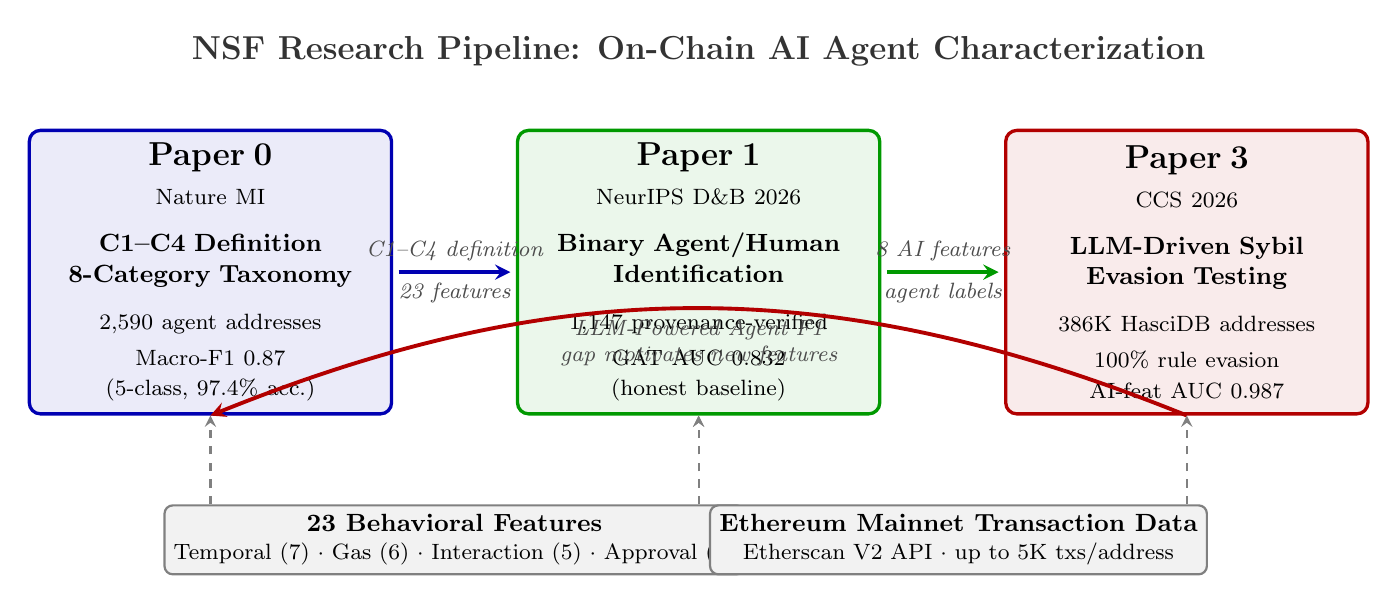
\begin{tikzpicture}[
    % Node styles
    paperbox/.style={
        rectangle,
        rounded corners=4pt,
        draw=#1,
        line width=1.2pt,
        fill=#1!8,
        minimum width=4.6cm,
        minimum height=3.6cm,
        text width=4.2cm,
        align=center,
        font=\small
    },
    databox/.style={
        rectangle,
        rounded corners=3pt,
        draw=black!50,
        line width=0.8pt,
        fill=black!5,
        minimum width=5cm,
        minimum height=0.8cm,
        align=center,
        font=\small
    },
    arrow/.style={
        ->,
        >=stealth,
        line width=1.4pt,
        color=#1
    },
    dataarrow/.style={
        ->,
        >=stealth,
        line width=0.8pt,
        dashed,
        color=black!50
    },
    label/.style={
        font=\footnotesize\itshape,
        text=black!70
    }
]

% ===== Paper boxes =====

% Paper 0
\node[paperbox=blue!70!black] (p0) at (0, 0) {
    \textbf{\large Paper 0}\\[3pt]
    {\footnotesize Nature MI}\\[6pt]
    \textbf{C1--C4 Definition}\\
    \textbf{8-Category Taxonomy}\\[6pt]
    {\footnotesize 2,590 agent addresses}\\[2pt]
    {\footnotesize Macro-F1 0.87}\\
    {\footnotesize (5-class, 97.4\% acc.)}
};

% Paper 1
\node[paperbox=green!60!black] (p1) at (6.2, 0) {
    \textbf{\large Paper 1}\\[3pt]
    {\footnotesize NeurIPS D\&B 2026}\\[6pt]
    \textbf{Binary Agent/Human}\\
    \textbf{Identification}\\[6pt]
    {\footnotesize 1,147 provenance-verified}\\[2pt]
    {\footnotesize GAT AUC 0.832}\\
    {\footnotesize (honest baseline)}
};

% Paper 3
\node[paperbox=red!70!black] (p3) at (12.4, 0) {
    \textbf{\large Paper 3}\\[3pt]
    {\footnotesize CCS 2026}\\[6pt]
    \textbf{LLM-Driven Sybil}\\
    \textbf{Evasion Testing}\\[6pt]
    {\footnotesize 386K HasciDB addresses}\\[2pt]
    {\footnotesize 100\% rule evasion}\\
    {\footnotesize AI-feat AUC 0.987}
};

% ===== Arrows between papers =====

\draw[arrow=blue!70!black] ([xshift=2pt]p0.east) -- ([xshift=-2pt]p1.west)
    node[midway, above, label] {C1--C4 definition}
    node[midway, below, label] {23 features};

\draw[arrow=green!60!black] ([xshift=2pt]p1.east) -- ([xshift=-2pt]p3.west)
    node[midway, above, label] {8 AI features}
    node[midway, below, label] {agent labels};

% ===== Feedback arrow P3 -> P0 =====

\draw[arrow=red!70!black, bend right=22] (p3.south) to
    node[midway, below, label, text width=6cm, align=center]
    {LLM-Powered Agent F1 gap motivates new features}
    (p0.south);

% ===== Shared data layer =====

\node[databox] (feat) at (3.1, -3.4) {
    \textbf{23 Behavioral Features}\\[-1pt]
    {\footnotesize Temporal (7) $\cdot$ Gas (6) $\cdot$ Interaction (5) $\cdot$ Approval (5)}
};

\node[databox] (data) at (9.5, -3.4) {
    \textbf{Ethereum Mainnet Transaction Data}\\[-1pt]
    {\footnotesize Etherscan V2 API $\cdot$ up to 5K txs/address}
};

% ===== Dashed arrows from data layer to papers =====

\draw[dataarrow] (feat.north -| p0) -- (p0.south);
\draw[dataarrow] (feat.north -| p1) -- (p1.south);
\draw[dataarrow] (data.north -| p1) -- (p1.south);
\draw[dataarrow] (data.north -| p3) -- (p3.south);

% ===== Title =====

\node[font=\large\bfseries, text=black!80] at (6.2, 2.8) {
    NSF Research Pipeline: On-Chain AI Agent Characterization
};

\end{tikzpicture}
\caption{Cross-paper pipeline. Paper~0 defines on-chain AI agents via four conditions (C1--C4) and validates an eight-category taxonomy on 2,590 addresses. Paper~1 uses the same 23 features for binary agent/human identification on 1,147 provenance-verified addresses (honest GAT AUC 0.832). Paper~3 tests whether LLM-driven Sybils can evade airdrop detectors; 8 AI-specific features from Paper~1 recover AUC 0.987 even after all HasciDB rules are defeated. The feedback arrow represents Paper~3's finding that the LLM-Powered Agent category (F1 = 0.528 in Paper~0) needs the 8 AI features to become distinguishable. Dashed arrows show shared data dependencies.}
\label{fig:pipeline}
\end{figure*}

% Requires: \usepackage{tikz} in the parent document
% =============================================================================
\begin{figure*}[t]
\centering
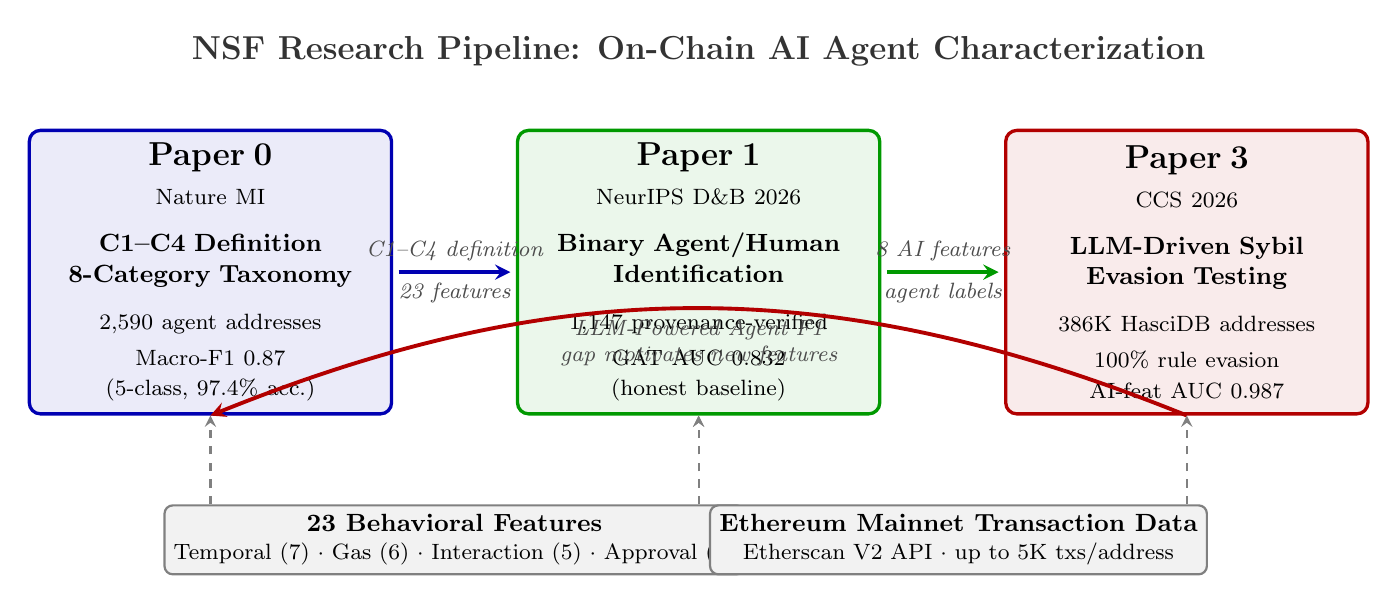
\begin{tikzpicture}[
    % Node styles
    paperbox/.style={
        rectangle,
        rounded corners=4pt,
        draw=#1,
        line width=1.2pt,
        fill=#1!8,
        minimum width=4.6cm,
        minimum height=3.6cm,
        text width=4.2cm,
        align=center,
        font=\small
    },
    databox/.style={
        rectangle,
        rounded corners=3pt,
        draw=black!50,
        line width=0.8pt,
        fill=black!5,
        minimum width=5cm,
        minimum height=0.8cm,
        align=center,
        font=\small
    },
    arrow/.style={
        ->,
        >=stealth,
        line width=1.4pt,
        color=#1
    },
    dataarrow/.style={
        ->,
        >=stealth,
        line width=0.8pt,
        dashed,
        color=black!50
    },
    label/.style={
        font=\footnotesize\itshape,
        text=black!70
    }
]

% ===== Paper boxes =====

% Paper 0
\node[paperbox=blue!70!black] (p0) at (0, 0) {
    \textbf{\large Paper 0}\\[3pt]
    {\footnotesize Nature MI}\\[6pt]
    \textbf{C1--C4 Definition}\\
    \textbf{8-Category Taxonomy}\\[6pt]
    {\footnotesize 2,590 agent addresses}\\[2pt]
    {\footnotesize Macro-F1 0.87}\\
    {\footnotesize (5-class, 97.4\% acc.)}
};

% Paper 1
\node[paperbox=green!60!black] (p1) at (6.2, 0) {
    \textbf{\large Paper 1}\\[3pt]
    {\footnotesize NeurIPS D\&B 2026}\\[6pt]
    \textbf{Binary Agent/Human}\\
    \textbf{Identification}\\[6pt]
    {\footnotesize 1,147 provenance-verified}\\[2pt]
    {\footnotesize GAT AUC 0.832}\\
    {\footnotesize (honest baseline)}
};

% Paper 3
\node[paperbox=red!70!black] (p3) at (12.4, 0) {
    \textbf{\large Paper 3}\\[3pt]
    {\footnotesize CCS 2026}\\[6pt]
    \textbf{LLM-Driven Sybil}\\
    \textbf{Evasion Testing}\\[6pt]
    {\footnotesize 386K HasciDB addresses}\\[2pt]
    {\footnotesize 100\% rule evasion}\\
    {\footnotesize AI-feat AUC 0.987}
};

% ===== Arrows between papers =====

\draw[arrow=blue!70!black] ([xshift=2pt]p0.east) -- ([xshift=-2pt]p1.west)
    node[midway, above, label] {C1--C4 definition}
    node[midway, below, label] {23 features};

\draw[arrow=green!60!black] ([xshift=2pt]p1.east) -- ([xshift=-2pt]p3.west)
    node[midway, above, label] {8 AI features}
    node[midway, below, label] {agent labels};

% ===== Feedback arrow P3 -> P0 =====

\draw[arrow=red!70!black, bend right=22] (p3.south) to
    node[midway, below, label, text width=6cm, align=center]
    {LLM-Powered Agent F1 gap motivates new features}
    (p0.south);

% ===== Shared data layer =====

\node[databox] (feat) at (3.1, -3.4) {
    \textbf{23 Behavioral Features}\\[-1pt]
    {\footnotesize Temporal (7) $\cdot$ Gas (6) $\cdot$ Interaction (5) $\cdot$ Approval (5)}
};

\node[databox] (data) at (9.5, -3.4) {
    \textbf{Ethereum Mainnet Transaction Data}\\[-1pt]
    {\footnotesize Etherscan V2 API $\cdot$ up to 5K txs/address}
};

% ===== Dashed arrows from data layer to papers =====

\draw[dataarrow] (feat.north -| p0) -- (p0.south);
\draw[dataarrow] (feat.north -| p1) -- (p1.south);
\draw[dataarrow] (data.north -| p1) -- (p1.south);
\draw[dataarrow] (data.north -| p3) -- (p3.south);

% ===== Title =====

\node[font=\large\bfseries, text=black!80] at (6.2, 2.8) {
    NSF Research Pipeline: On-Chain AI Agent Characterization
};

\end{tikzpicture}
\caption{Cross-paper pipeline. Paper~0 defines on-chain AI agents via four conditions (C1--C4) and validates an eight-category taxonomy on 2,590 addresses. Paper~1 uses the same 23 features for binary agent/human identification on 1,147 provenance-verified addresses (honest GAT AUC 0.832). Paper~3 tests whether LLM-driven Sybils can evade airdrop detectors; 8 AI-specific features from Paper~1 recover AUC 0.987 even after all HasciDB rules are defeated. The feedback arrow represents Paper~3's finding that the LLM-Powered Agent category (F1 = 0.528 in Paper~0) needs the 8 AI features to become distinguishable. Dashed arrows show shared data dependencies.}
\label{fig:pipeline}
\end{figure*}
